% sample template

\documentclass[12pt]{article}
\usepackage[spanish]{babel}
\usepackage{natbib}
\usepackage{url}
\usepackage[utf8x]{inputenc}
\usepackage{indentfirst}
\usepackage{amsmath}
\usepackage{graphicx}
\graphicspath{{images/}}
\usepackage{float} % allows to place the image or tables where we want to.
\usepackage{fancyhdr}
\usepackage{vmargin}
\setlength{\parskip}{3mm} % length between paragraphs
\usepackage{subfigure} % allows to include subfigures
\setpapersize{A4} % A4 format
\usepackage{color}
\definecolor{gray97}{gray}{.97}
\definecolor{gray75}{gray}{.75}
\definecolor{gray45}{gray}{.45}
\setmarginsrb{3 cm}{2.5 cm}{3 cm}{2.5 cm}{1 cm}{1.5 cm}{1 cm}{1.5 cm}

\title{Blendify: Lenguaje para la definición de simulaciones físicas}			% Title
\author{Alberto Aranda García \\ Cristian Gómez Portes \\ Daniel Pozo Romero \\ Eduardo Sánchez López}				% Author
\date{\today}				%Current  Date

\makeatletter
\let\thetitle\@title
\let\theauthor\@author
\let\thedate\@date
\makeatother

\pagestyle{fancy}
\fancyhf{}
\lhead{\thetitle}
\cfoot{\thepage}

\begin{document}

%%%%%%%%%%%%%%%%%%%%%%%%%%%%%%%%%%%%%%%%%%%%%%%%%%%%%%%%%%%%%%%%%%%%%%%%%%%%%%%%%%%%%%%%%

\begin{titlepage}
	\centering
    \vspace*{0.5 cm}
    
\includegraphics[scale = 0.1]{informatica.png}\\[1.0 cm]										% University Logo
    \textsc{\LARGE Universidad de Castilla-La Mancha\newline\newline Escuela Superior De Informática}\\[2.0 cm]		% University Name
	\textsc{\Large Memoria de Prácticas}\\[0.5 cm]												% Subject
	\rule{\linewidth}{0.2 mm} \\[0.4 cm]
	{ \huge \bfseries \thetitle}\\
	\rule{\linewidth}{0.2 mm} \\[1.5 cm]
	
	\begin{minipage}{0.4\textwidth}
		\begin{center} \large
			\emph{Autores:}\\
			\theauthor\\
			\vspace*{1 cm}
			\emph{Fecha:}\\
			\thedate\\
			\end{center}
        
	\end{minipage}\\[2 cm]
	
\end{titlepage}

%%%%%%%%%%%%%%%%%%%%%%%%%%%%%%%%%%%%%%%%%%%%%%%%%%%%%%%%%%%%%%%%%%%%%%%%%%%%%%%%%%%%%%%%%

\tableofcontents
\pagebreak

%%%%%%%%%%%%%%%%%%%%%%%%%%%%%%%%%%%%%%%%%%%%%%%%%%%%%%%%%%%%%%%%%%%%%%%%%%%%%%%%%%%%%%%%%

\section{Presentación del problema}

Dentro de la enseñanza de Física, la visualización de los problemas es una herramienta muy importante para que los estudiantes comprendan mejor los conceptos teóricos existentes tras ellos. En este contexto, la simulación es una opción que lleva disponible durante años, pero que está siendo muy infrautilizada.

Esto tiene una fácil explicación: la mayoría de programas de generación de simulaciones físicas imponen interfaces gráficas que requieren una inversión de tiempo grande por parte del usuario: partiendo de un enunciado textual de un problema, el usuario, que puede ser tanto un profesor como un estudiante de física, se ve obligado a traducirlo manualmente a un formato gráfico, lidiando muchas veces con interfaces de usuario tediosas que hacen perder mucho tiempo, tanto para aprenderlas, como por las operaciones repetitivas que deben realizarse. 

Lo ideal sería que, a partir de un enunciado de un problema, fuese posible la generación automática de su simulación. Dejando de lado las dificultades que el Procesado de Lenguaje Natural supone (aún dentro de un dominio tan acotado), una primera aproximación puede ser la creación de un lenguaje con un poder expresivo similar al de los enunciados de problemas, al que sea lo más sencillo posible traducir (para un humano) dichos enunciados escritos originalmente en lenguaje natural.

Como plataforma de simulaciones físicas, vamos a considerar Blender, ya que incorpora, entre muchas otras funcionalidades, un motor de físicas muy potente, y, tanto o más importante, una API para Python que expone prácticamente todas las funcionalidades del programa.

Para nuestra práctica, por tanto, consideramos la definición de un lenguaje que permita escribir simulaciones físicas, y la construcción de un procesador de lenguajes que lo traduzca a código Python que use la API de Blender, que posteriormente podrá ser interpretado por este programa para generar una simulación. Nuestro objetivo principal, pues, es simplificar al máximo posible la generación de simulaciones que de otra forma serían muy tediosas de realizar.

\section{Descripción del lenguaje}

Como se ha dicho anteriormente, nuestro lenguaje, llamado X, deberá tener el mismo poder expresivo los enunciados de problemas, y posiblemente, permitir definir ciertos hechos sobre el contexto que se dan por supuesto (tipo de problema, dimensionalidad, etc.). Si analizamos la estructura de los enunciados, nos encontramos con que, primero, se nos da información sobre los elementos que intervienen en el problema (cubo, esfera, polea, rampa, electrón, planeta…) y sus parámetros (masa, velocidad, fuerzas que actúan sobre este…); posteriormente, se suele dar una condición que podemos considerar como de parada de la simulación, y una pregunta (que podemos felizmente obviar) sobre algún parámetro de un elemento en determinado momento. Nuestro lenguaje, pues, deberá permitir declarar diferentes objetos y sus correspondientes atributos, así como ciertos parámetros globales que afecten a toda la simulación, alguna condición de parada, y posiblemente, información sobre qué quiere hacer el usuario con la simulación (ejecutarla, generar una animación, etc.).

\subsection{Tabla de Tokens}


\begin{figure}[H] % we need to specify the letter "H" to put the image in the right place
\centering
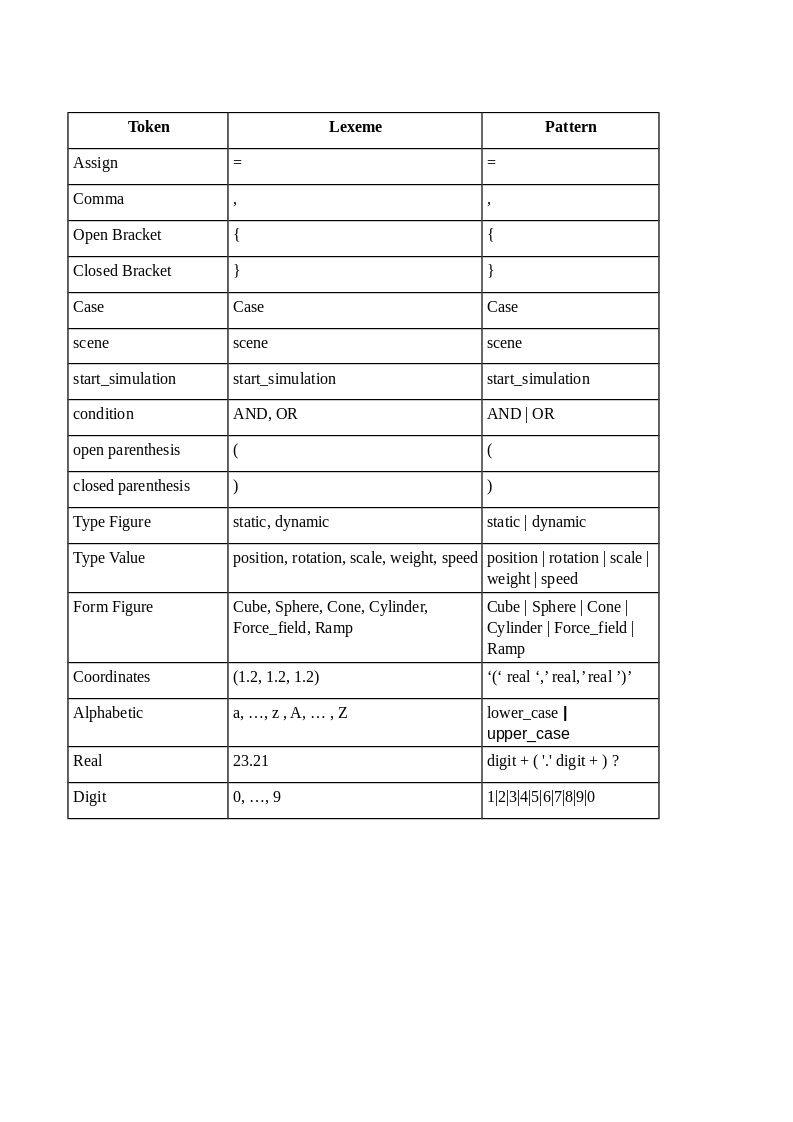
\includegraphics[width=\linewidth]{TablaTokens.jpg}
\end{figure}


\end{document}